\chapter{Deep Learning for Smart Agriculture}

\section{Introduction}
Deep learning and computer vision have become indispensable tools in modern agriculture, enabling automated, high-precision analysis of crop health, disease detection, and pest management. By leveraging convolutional neural networks (CNNs), these technologies can process vast amounts of visual data from drone imagery to ground-based cameras, identifying subtle patterns indicative of wheat diseases. This shift from manual scouting to AI-driven monitoring improves scalability, reduces human error, and supports timely interventions, ultimately enhancing yield and sustainability.

In this chapter, we establish the foundational concepts of deep learning and computer vision as applied to agricultural challenges. We begin by examining the core principles of CNNs and their role in feature extraction from crop imagery. Next, we explore transfer learning techniques, which allow pre-trained models to adapt to agricultural datasets with limited labeled examples. The chapter then discusses object detection methods critical for localizing diseases and pests in field conditions. Finally, we address the practical challenges of implementing these solutions, including data variability, model scalability, and real-world deployment constraints in agricultural settings.

\section{Overview of Smart Agriculture}
Smart agriculture integrates advanced technologies such as the Internet of Things (IoT), artificial intelligence (AI), and big data analytics to enhance farming efficiency and sustainability. By leveraging real-time data from sensors, drones, and satellite imagery, smart agricultural systems enable precise monitoring of soil conditions, crop health, and environmental factors \parencite{garg2023smart}.
Machine learning and deep learning techniques, particularly computer vision, play a crucial role in automating disease detection, pest control, and yield prediction. These AI-driven solutions reduce dependency on manual labor, optimize resource usage, and facilitate data-driven decision-making. The adoption of smart agriculture not only improves productivity but also promotes sustainable farming practices, addressing global food security challenges \parencite{garg2023smart}.

\section{Deep Learning Fundamentals}
In this section, we introduce the core principles of deep learning, focusing on deep neural networks (DNNs) and their role in learning complex patterns from data. We explore the structure and components of neural networks, the learning process, optimization techniques, and model evaluation methods. Additionally, we highlight regularization strategies to prevent overfitting.

\subsection{Deep Neural Network Basics (DNN)}
Neural networks form the backbone of deep learning, enabling machines to learn patterns and make predictions from data. Inspired by the structure of the human brain, these networks consist of interconnected layers of artificial neurons that hierarchically process information.

\subsubsection{Definition of DNN}

Before defining deep neural networks, we first need to understand two essential components: 
\begin{itemize}
    \item \textbf{Artificial neuron}: An artificial neuron is the basic building block of artificial neural networks, designed based on the structure and functionality of biological neurons. It receives weighted inputs, processes them through a transfer function, and outputs the result. The artificial neuron model simplifies the biological process where information is received through dendrites, processed in the soma, and transmitted via the axon, as shown in Figure~\ref{fig:figure01} \parencite{krenker2011introduction}.
    
    \item \textbf{Layer}: A layer in a neural network is a set of neurons that perform a specific operation on the data \parencite{bengio2017deep}.
\end{itemize}

\begin{figure}[H] % 'H' needs \usepackage{float}
    \centering
    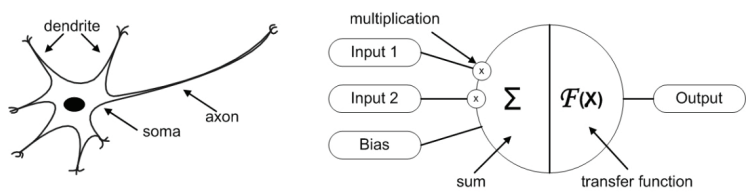
\includegraphics[width=0.6\textwidth]{chapters/chapter1/images/Figure01.png}
    \caption{Biological Neuron Structure and Its Mathematical Model Representation \parencite{krenker2011introduction}.}
    \label{fig:figure01}
\end{figure}


By combining multiple layers of interconnected artificial neurons, we arrive at the concept of a Deep Neural Network (DNN). \parencite{A DNN is a neural network} that contains multiple hidden layers between the input and output layers. These additional layers enable the network to learn complex patterns and high-level features from data. Each layer transforms its input into a more abstract representation, improving the network’s ability to recognize intricate structures and relationships \parencite{li2021water}.
\subsubsection{Structure of DNN}
A neural network consists of three main layers \parencite{ren2023review}:

\noindent
\textbf{The input layer:} Represents the features of the input data, such as pixel values in an image, denoted as a vector 
\[
X = [x_1, x_2, \dots, x_n].
\]

\noindent
\textbf{The hidden layers:} Process this input using weighted connections and biases, computed as:
\[
z = W \cdot X + b_z \tag{1}
\]
\[
F(z) = a \tag{2}
\]
where:
\begin{itemize}
    \item $W$ is the weight matrix,
    \item $b$ is the bias vector,
    \item $z$ is the pre-activation value,
    \item $F(z)$ is the activation function applied to $z$.
\end{itemize}

Each neuron in the hidden layers applies an activation function to capture complex patterns.

\noindent
\textbf{The output layer:} Generates the network's prediction, with the number of neurons corresponding to the specific task, such as one neuron for binary classification (as presented in Figure~\ref{fig:figure02}) or multiple neurons for multiclass classification.



\begin{figure}[H] % 'H' needs \usepackage{float}
    \centering
    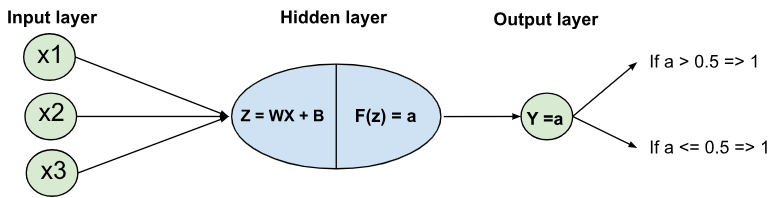
\includegraphics[width=0.6\textwidth]{chapters/chapter1/images/Figure02.png}
    \caption{The structure of a Neural Network in the binary classification task.}
    \label{fig:figure02}
\end{figure}

\subsubsection{Activation Functions}
An activation function (AF) is a mathematical function applied to a neuron's output in a neural network to introduce non-linearity. Without an activation function, a neural network with multiple layers would behave like a single-layer perceptron, limiting its ability to model complex relationships \parencite{dubey2022activation}. Activation functions decide whether a neuron should be activated based on its input. 

Table \ref{tab:activation-functions} summarizes the most commonly used activation functions, their formulas, ranges, and typical use cases in deep neural networks.



\begin{table}[htbp]
    \caption{Common Activation Functions in Deep Learning (Dubey et al., 2022)}
    \centering
    \resizebox{\textwidth}{!}{%
    \begin{tabular}{|p{3cm}|p{4.5cm}|p{3cm}|p{3.5cm}|}
    \hline
    \textbf{Activation Function} & \textbf{Formula} & \textbf{Range} & \textbf{Usage} \\
    \hline
    Sigmoid                      & $\frac{1}{1+e^{-x}}$         & [0, 1]               & Commonly used in binary classification problems, especially in the output layer of models predicting probabilities. \\
    \hline
    Tanh (Hyperbolic Tangent)     & $\tanh(x) = \frac{e^{x} - e^{-x}}{e^{x} + e^{-x}}$ & [-1, 1] & Often used in hidden layers of neural networks, as it outputs values centered around zero, which helps in reducing bias during optimization. \\
    \hline
    ReLU (Rectified Linear Unit)  & $\text{max}(0, x)$            & [0, $\infty$)        & Widely used in hidden layers of deep neural networks due to its simplicity and effectiveness in handling the vanishing gradient problem. \\
    \hline
    Softmax                      & $\text{Softmax}(x_i) = \frac{e^{x_i}}{\sum_j e^{x_j}}$ & (0, 1) (outputs sum to 1) & Used in the output layer for multi-class classification. \\
    \hline
    \end{tabular}%
    }
    \label{tab:activation-functions}
\end{table}


    
\subsection{Learning Process in Deep Neural Networks}

In the information processing flow within an artificial neuron, several elements, known as parameters, are learned from the training data. These parameters include \parencite{Kelleher2019}:
\begin{itemize}
    \item \textbf{Weights}: Weights control the amount of each input feature that passes through the neuron. They represent the coefficients of the connections between neurons in the layers of a neural network. Weights are essential for determining the influence of each input on the output.
    
    \item \textbf{Biases}: Biases are values added to the outputs of the neurons before applying the activation function. They allow the network to shift the activation function, providing more flexibility to the model.
\end{itemize}

The learning process in neural networks involves training the model to map input data to desired outputs. This is achieved through the mechanisms of forward propagation and backward propagation, along with optimization techniques that refine the network's parameters (weights and biases) to minimize the error \parencite{Kelleher2019}:
\begin{itemize}
    \item \textbf{Forward Propagation}: In forward propagation, the input data passes through the network layer by layer. Each neuron in a layer performs a weighted sum of its inputs, applies an activation function, and passes the result to the next layer. The process continues until the output layer is reached and a prediction is made.
    
    \item \textbf{Backward Propagation}: Backward propagation (or backpropagation) is used to update the network's weights. After calculating the error (the difference between the predicted and actual output), the error is propagated back through the network. The weights are adjusted based on the gradient of the error with respect to each weight, using optimization algorithms like gradient descent.
\end{itemize}

Figure \ref{fig:figure03} below provides a visual representation of the learning process in a neural network, illustrating the flow of information from the input layer through multiple hidden layers to the output layer.


\begin{figure}[H] % 'H' needs \usepackage{float}
    \centering
    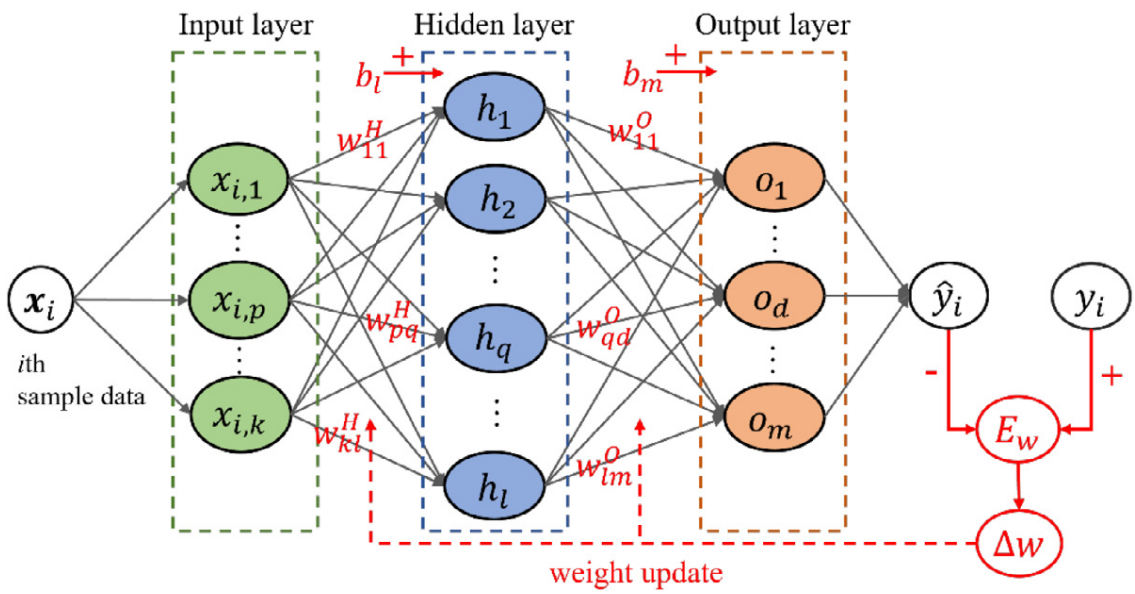
\includegraphics[width=0.6\textwidth]{chapters/chapter1/images/Figure03.png}
    \caption{The structure of the DNN \cite{ren2023review}.}
    \label{fig:figure03}
\end{figure}



\subsection{Model Training Concepts}

Effective model training ensures that neural networks learn patterns in data while minimizing errors. This section highlights essential components of the training process.

\paragraph{Loss Functions} 
Loss functions quantify the error between predicted and actual values, guiding weight updates during optimization \parencite{alzubaidi2021review}. Common loss functions include:
\begin{itemize}
    \item \textbf{Cross-Entropy Loss}: Used for classification tasks to measure the divergence between predicted probabilities and true labels.
    \item \textbf{Mean Squared Error (MSE)}: Applied in regression, computing the average squared difference between predicted and actual values.
\end{itemize}

\paragraph{Overfitting Prevention}
Overfitting occurs when a model learns noise from training data, reducing generalization to unseen data. Common techniques to mitigate overfitting include:
\begin{itemize}
    \item \textbf{Dropout}: Randomly deactivate neurons during training to enhance robustness.
    \item \textbf{Data Augmentation}: Transform training samples (e.g., rotation, scaling) to increase dataset diversity.
\end{itemize}

\paragraph{Batch Normalization}
Batch normalization stabilizes training by normalizing inputs across a mini-batch, reducing internal covariate shift and accelerating convergence.



\subsection{Optimization Methods and Strategies}
Optimization techniques in deep learning are methods used to minimize the loss function during training, improving the model’s accuracy. These techniques adjust the model's weights and biases iteratively to find the optimal set of parameters that reduces the error between predicted and actual values \parencite{alzubaidi2021review}.

Different optimizers are used to update model weights efficiently:

\begin{itemize}
    \item \textbf{Stochastic Gradient Descent (SGD):} Updates weights based on a small subset (batch) of training data, improving computational efficiency.
    \item \textbf{Adam (Adaptive Moment Estimation):} Combines momentum and adaptive learning rates for faster and more stable convergence.
    \item \textbf{RMSprop:} Uses an adaptive learning rate to prevent oscillations and improve performance on non-stationary objectives.
\end{itemize}

However, an important consideration in optimization is how to set the learning rate throughout training. While optimizers control how weights are updated, learning rate scheduling adjusts the learning rate over time to further optimize training.

Different scheduling strategies can be used in conjunction with optimizers \parencite{zhao2019learningrate}:

\begin{itemize}
    \item \textbf{Step Decay:} Reduces the learning rate at fixed intervals, allowing for more stable training as the model reaches its optimal solution.
    \item \textbf{Exponential Decay:} Gradually decreases the learning rate across epochs, promoting finer adjustments to the model parameters as the training progresses.
    \item \textbf{Cyclic Learning Rates:} Alternates between a minimum and maximum learning rate, which helps the model escape local minima and enhances exploration of the parameter space.
\end{itemize}

By combining these scheduling strategies with optimization techniques, the training process can become more efficient and effective, leading to faster and more reliable convergence.






\subsection{Model Evaluation and Validation}

Once a model is trained, it is crucial to assess its performance and ensure that it generalizes well to unseen data. This process is known as \textbf{model evaluation and validation}. The primary goal is to measure how well the model performs and to identify any potential overfitting or underfitting issues.

To evaluate a model’s performance, several metrics can be used depending on the type of task (classification, regression, etc.) \parencite{ketkar2017deep}:
\begin{itemize}
    \item \textbf{Accuracy:} For classification tasks, accuracy measures the proportion of correct predictions out of all predictions made. However, accuracy alone can be misleading in imbalanced datasets.
    \item \textbf{Precision and Recall:} In imbalanced classification problems, precision (the proportion of true positive results among all positive predictions) and recall (the proportion of true positive results among all actual positives) are often used in conjunction to provide a clearer view of the model's performance.
    \item \textbf{F1-Score:} The harmonic mean of precision and recall; F1-score balances the two metrics and is especially useful when dealing with imbalanced datasets.
    \item \textbf{Mean Squared Error (MSE):} For regression tasks, MSE calculates the average of the squared differences between predicted and actual values. It penalizes large errors more significantly than smaller ones.
    \item \textbf{R-squared (R²):} For regression, this metric indicates how well the model explains the variability in the data, with a value closer to 1 suggesting a better fit.
\end{itemize}


\section{Deep Learning Approaches}

Deep learning encompasses a variety of learning paradigms that enable models to extract complex patterns from large volumes of data. These approaches differ based on the nature of the data, the availability of labels, and the interaction mechanisms with the environment. This section presents the four main categories of deep learning methods \parencite{alzubaidi2021review}:

\begin{itemize}
    \item \textbf{Deep Supervised Learning:} This approach involves training a neural network using a labeled dataset, where each input image (e.g., leaf with visible symptoms) is paired with its correct label (e.g., disease type). The model learns to minimize the error between its predictions and the true labels using backpropagation and optimization algorithms. Techniques include Convolutional Neural Networks (CNNs) for spatial feature extraction, Deep Neural Networks (DNNs), and Recurrent Neural Networks (RNNs) like LSTMs and GRUs when dealing with sequential data.
    
    \item \textbf{Deep Semi‐Supervised Learning:} Semi-supervised learning combines a small labeled dataset with a larger pool of unlabeled data, which is common in agricultural settings where annotating plant diseases is costly and time-consuming. Methods like Generative Adversarial Networks (GANs) can generate synthetic labeled images, while RNNs, LSTMs, and Deep Reinforcement Learning (DRL) can help model complex data behavior.
    
    \item \textbf{Deep Unsupervised Learning:} Unsupervised learning aims to extract meaningful patterns from unlabeled data, such as grouping similar plant images or identifying features without predefined classes. Popular methods include Autoencoders for dimensionality reduction, Restricted Boltzmann Machines, and clustering algorithms. These are useful in exploratory stages or feature extraction before applying a classifier.
    
    \item \textbf{Deep Reinforcement Learning (DRL):} In DRL, models learn optimal actions through trial and error by interacting with an environment. This could include real-time monitoring systems in agriculture, like automated disease response tools or robotic weeders. Unlike supervised learning, DRL does not require labeled data but instead uses reward signals to adjust its strategy over time.
\end{itemize}

\section{Convolutional Neural Networks (CNNs) for Plant Disease Classification}

Convolutional Neural Networks (CNNs) have revolutionized image-based plant disease classification by automatically extracting hierarchical features from agricultural images. Unlike traditional machine learning approaches that rely on handcrafted features, CNNs learn spatial patterns directly from raw images, improving classification accuracy. Their ability to recognize disease symptoms from leaf textures and color variations makes them particularly effective in precision agriculture. This section explores the fundamental components of CNNs, their advantages in agricultural applications, and their limitations when applied independently.

\subsection{Fundamentals of CNNs}
Convolutional Neural Networks (CNNs) consist of multiple layers designed to process and learn spatial hierarchies from image data (see Figure~\ref{fig:figure04}). Their architecture typically includes \parencite{alzubaidi2021review}:

\begin{itemize}
    \item \textbf{Convolutional Layers:} Extract features using small filters (kernels) that detect edges, textures, and patterns. A kernel is a grid of values (weights) initialized randomly at the start of training and adjusted through learning to identify important features.
     
     \begin{itemize}
        \item \textbf{Input and Kernel Dimensions:} In a CNN layer, each input $x$ is structured in three dimensions: height, width, and depth. The depth corresponds to the number of channels (e.g., an RGB image has three channels). Similarly, the kernels are also three-dimensional, with spatial dimensions (height and width) and a depth matching the input channels. Each kernel has shared parameters---a set of weights and a bias. When applied to the input, these kernels generate a corresponding set of feature maps. These kernels establish local connections by interacting only with small regions of the input at a time, allowing the network to extract patterns such as edges and textures by computing dot products across these regions.
        \item \textbf{Convolutional Operation:} The convolutional process begins by sliding the kernel across the input image in both horizontal and vertical directions. At each location, the dot product between the kernel and the overlapping region of the input is computed, producing a scalar value that becomes part of the resulting feature map. As this process is repeated across the image, a full feature map is constructed, highlighting areas where the kernel detects specific patterns. Parameters such as stride (controlling how far the kernel moves at each step) and padding (adding borders to the input to preserve edge information) affect the size and coverage of the output feature map. These concepts are illustrated in Figure~\ref{fig:figure05}.
     \end{itemize}   
    
     \begin{figure}[H] % 'H' needs \usepackage{float}
        \centering
        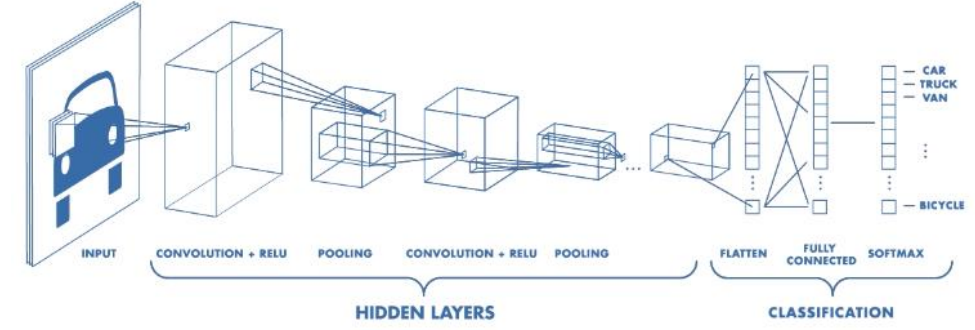
\includegraphics[width=0.6\textwidth]{chapters/chapter1/images/Figure04.png}
        \caption{Architecture of CNN \cite{purwono2022understanding}.}
        \label{fig:figure04}
    \end{figure}
    
    \begin{figure}[H] % 'H' needs \usepackage{float}
        \centering
        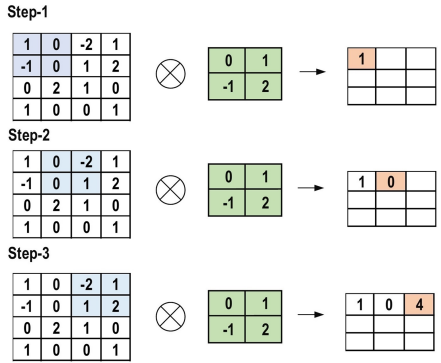
\includegraphics[width=0.6\textwidth]{chapters/chapter1/images/Figure05.png}
        \caption{The primary calculations executed at each step of the convolutional layer \parencite{alzubaidi2021review}.}
        \label{fig:figure05}
    \end{figure}

    \item \textbf{Pooling Layers:} Pooling layers are used to reduce the spatial dimensions of feature maps while preserving the most important information. This reduction helps lower the computational cost and minimizes the risk of overfitting by simplifying the data representation. The pooling operation works by sliding a small filter over the feature map and applying a summary function within each local region (Figure~\ref{fig:figure06}). Common types of pooling include:
    \begin{itemize}
        \item \textbf{Max Pooling:} Selects the maximum value in each region.
        \item \textbf{Average Pooling:} Calculates the average value of the region.
        \item \textbf{Global Average Pooling:} Computes the average across the entire feature map.
     \end{itemize}  
    
     \begin{figure}[H] % 'H' needs \usepackage{float}
        \centering
        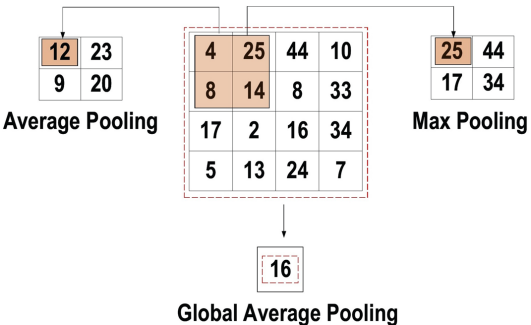
\includegraphics[width=0.6\textwidth]{chapters/chapter1/images/Figure06.png}
        \caption{Three types of pooling operations \parencite{alzubaidi2021review}.}
        \label{fig:figure06}
    \end{figure}
 
    \item \textbf{Activation Functions:} Introduce non-linearity to help the network learn complex patterns. They must also be differentiable to enable backpropagation during training. CNNs commonly utilize the following activation functions: ReLU (Rectified Linear Unit), Sigmoid, Softmax, and Tanh.
    \item \textbf{Fully Connected Layers:} The Fully Connected (FC) layer is typically found at the end of a CNN architecture and serves as the classifier. In this layer, each neuron is connected to all neurons from the previous layer, following the fully connected approach. It operates similarly to a conventional multi-layer perceptron (MLP) network, which is a type of feed-forward artificial neural network (ANN). The input to the FC layer is a vector created from the feature maps after flattening, which comes from the last pooling or convolutional layer. The output of the FC layer represents the final result of the classification task.
    
\end{itemize}

Figure~\ref{fig:figure07} below illustrates the general structure of a Convolutional Neural Network (CNN), highlighting its layers, which work together to extract and classify features from input images.

\begin{figure}[H] % 'H' needs \usepackage{float}
    \centering
    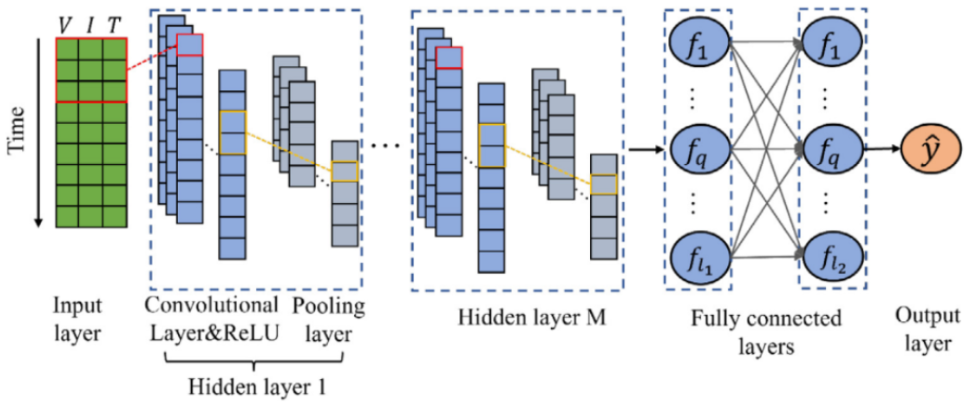
\includegraphics[width=0.6\textwidth]{chapters/chapter1/images/Figure07.png}
    \caption{The structure of the CNN \parencite{crocioni2020li}.}
    \label{fig:figure07}
\end{figure}


\subsection{CNN Architectures for Image Classification}
Over the past decade, numerous Convolutional Neural Network (CNN) architectures have been developed, each introducing unique design principles to improve accuracy, efficiency, and scalability. In the context of image classification, especially for tasks such as plant disease detection, the choice of architecture can significantly influence performance depending on the dataset size, complexity, and computational constraints.
This section presents an overview of some of the most influential and widely used CNN architectures:
\subsubsection{Visual geometry group network (VGGNet)}
Proposed by Simonyan and Zisserman, VGGNet is a convolutional neural network (CNN) architecture widely recognized for its simplicity and strong performance in image recognition tasks.

VGG is characterized by its deep architecture, typically comprising 16 to 19 layers, which significantly enhances its representational power compared to earlier models like ZFNet and AlexNet. One of its key innovations is the replacement of large convolutional filters (such as $11 \times 11$ or $5 \times 5$) with multiple stacked $3 \times 3$ filters. This strategy maintains an equivalent receptive field while reducing the number of parameters and improving computational efficiency.

In addition, VGG uses $1 \times 1$ convolutions to control the model’s complexity and includes max pooling layers to progressively reduce the spatial dimensions of the feature maps, as illustrated in Figure~\ref{fig:figure08}.

Despite its effectiveness, a major drawback of VGGNet is its high computational cost, with around 140 million parameters \parencite{alzubaidi2021review}. Nonetheless, its reliable feature extraction capabilities have made it a popular choice in applications like plant disease classification, especially for detecting early-stage or visually subtle symptoms.


\begin{figure}[H] % 'H' needs \usepackage{float}
    \centering
    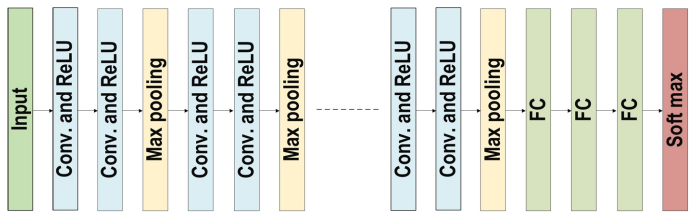
\includegraphics[width=0.6\textwidth]{chapters/chapter1/images/Figure08.png}
    \caption{The architecture of VGG \parencite{alzubaidi2021review}.}
    \label{fig:figure08}
\end{figure}

\subsubsection{Inception Net (GoogLeNet)}
Inception Net, introduced by Szegedy et al., uses Inception modules that apply multiple convolutional filters ($1 \times 1$, $3 \times 3$, $5 \times 5$) in parallel, followed by concatenation (see Figure~\ref{fig:figure09}). This design captures multi-scale information efficiently while reducing computational cost. The architecture has been successfully applied in plant phenotyping and classification of complex disease patterns.

It replaced standard convolutional layers with micro-neural networks and regulated computation through $1 \times 1$ convolutions as bottleneck layers. Sparse connections addressed redundant information by selectively connecting input and output channels, while the global average pooling (GAP) layer reduced parameters from 40 million to just 5 million, enhancing efficiency. Additional features included the RmsProp optimizer, batch normalization, and auxiliary learners to accelerate convergence \parencite{alzubaidi2021review}.



\begin{figure}[H] % 'H' needs \usepackage{float}
    \centering
    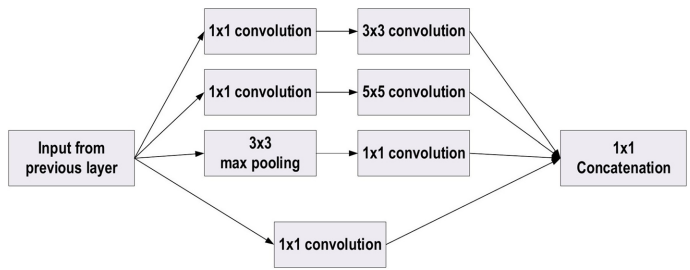
\includegraphics[width=0.6\textwidth]{chapters/chapter1/images/Figure09.png}
    \caption{The basic structure of Google Block \parencite{alzubaidi2021review}.}
    \label{fig:figure09}
\end{figure}

\subsubsection{Xception Net}

The Xception model is an extension of the Inception architecture that replaces standard convolutions with depth-wise separable convolutions, significantly improving efficiency. It has been shown to outperform Inception in many tasks, especially with high-resolution agricultural images, by learning spatial and cross-channel correlations separately.

The core concept behind Xception is the modification of the traditional Inception block by making it wider and replacing the standard $3 \times 3$ convolution followed by a $1 \times 1$ convolution with depthwise separable convolutions, which reduces computational complexity while enhancing performance \parencite{alzubaidi2021review}. An illustration of the basic Xception block structure is presented in Figure~\ref{fig:figure10}.


\begin{figure}[H] % 'H' needs \usepackage{float}
    \centering
    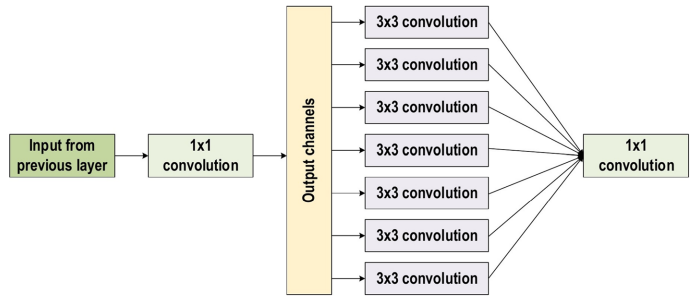
\includegraphics[width=0.6\textwidth]{chapters/chapter1/images/Figure10.png}
    \caption{The basic block diagram for the Xception block architecture \parencite{alzubaidi2021review}.}
    \label{fig:figure10}
\end{figure}

\subsubsection{Residual Networks (ResNet)}
ResNet is a deep convolutional neural network architecture developed to facilitate the training of very deep networks, ranging from 18 to 152 layers, by introducing the concept of residual learning through shortcut (or skip) connections that bypass one or more layers.

These residual connections address the degradation problem that often occurs in deeper networks, where increasing depth leads to performance saturation or even degradation. By enabling gradients to flow more efficiently, ResNet makes it easier for the network to learn identity mappings or residual functions, simplifying the overall training process.

The output of a residual block is defined as:
\begin{equation}
    H(x) = F(x) + x  \tag{3}
\end{equation}

Where:
\begin{itemize}
    \item $H(x)$: the output of the residual block,
    \item $F(x)$: the residual function to be learned,
    \item $x$: the input passed through the shortcut connection.
\end{itemize}

This formulation (3) makes it easier to optimize deep networks by learning the difference (residual) between the desired mapping and the identity. Additionally, it helps increase the rank of the weight matrices, enhancing the network’s expressiveness and preventing performance degradation.

An illustration of the residual module structure is provided in Figure~\ref{fig:figure11}.


\begin{figure}[H] % 'H' needs \usepackage{float}
    \centering
    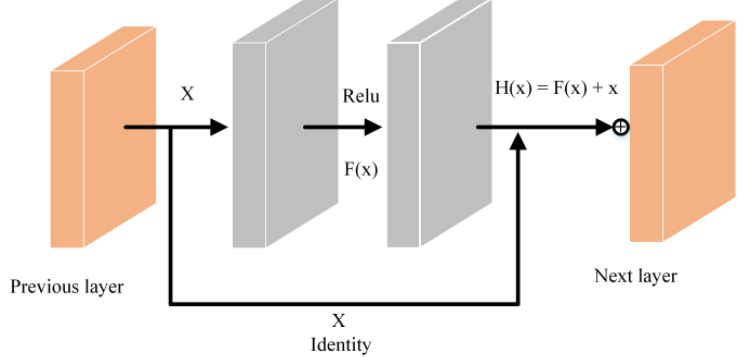
\includegraphics[width=0.6\textwidth]{chapters/chapter1/images/Figure11.png}
    \caption{Residual module diagram \parencite{fang2023lightweight}.}
    \label{fig:figure11}
\end{figure}

\subsubsection{DenseNet}

DenseNet is a convolutional neural network architecture that introduces the concept of dense connectivity, in which each layer is directly connected to every other layer in a feed-forward fashion, as illustrated in Figure~\ref{fig:figure12}. This unique design enables feature reuse, enhances gradient flow, and significantly reduces the number of parameters compared to traditional CNNs.

Inspired by ResNet and Highway Networks, DenseNet addresses a key limitation in ResNet, where each layer maintains isolated weights and where certain transformations contribute minimal new information. In contrast, DenseNet concatenates the outputs of all preceding layers and feeds them as input to each subsequent layer.

In a DenseNet with $l$ layers, the number of direct connections between layers is given by:
\[
\text{Number of connections} = \frac{l(l+1)}{2} \tag{4}
\]

This connectivity pattern facilitates richer feature propagation, introduces a regularization effect, and helps mitigate the vanishing gradient problem, thus improving training efficiency and model generalization \parencite{alzubaidi2021review}.

Despite the computational cost introduced by the accumulation of feature maps, DenseNet has shown exceptional performance in fine-grained classification tasks, such as distinguishing between subtly different plant disease symptoms, particularly in scenarios with limited training data.

\begin{figure}[H] % 'H' needs \usepackage{float}
    \centering
    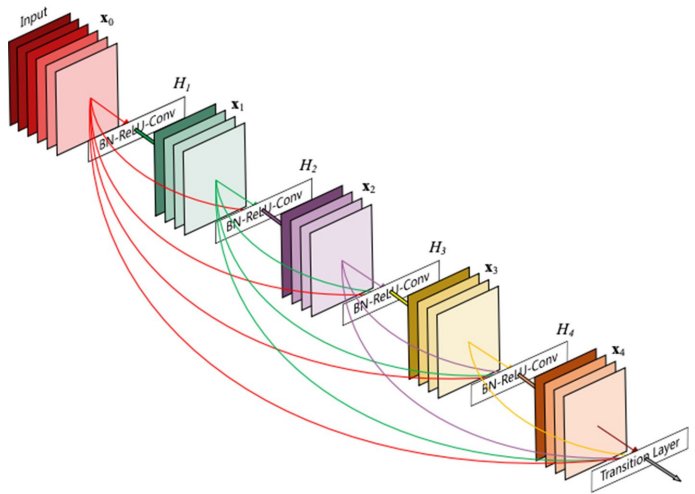
\includegraphics[width=0.6\textwidth]{chapters/chapter1/images/Figure12.png}
    \caption{The architecture of DenseNet Network \parencite{alzubaidi2021review}.}
    \label{fig:figure12}
\end{figure}


\subsubsection{EfficientNet}


EfficientNet is a family of convolutional neural networks developed by Google AI that introduces a compound scaling method to efficiently scale deep learning models. Traditional approaches often scale models arbitrarily in one of three dimensions: depth (number of layers), width (number of channels), or input resolution. However, EfficientNet proposes a more balanced and systematic strategy, where all three dimensions are scaled simultaneously and proportionally using a fixed set of scaling coefficients. This compound approach maintains model efficiency while significantly boosting accuracy.

The baseline model, EfficientNet-B0 (see Figure~\ref{fig:figure13}), is built using Neural Architecture Search (NAS) to optimize both performance and efficiency. Larger variants (B1 to B7) are derived by uniformly scaling the baseline model using the compound scaling principle. This results in models that achieve state-of-the-art performance on image classification tasks with dramatically fewer parameters and lower computational cost compared to earlier architectures like ResNet or Inception.

\begin{figure}[H] % 'H' needs \usepackage{float}
    \centering
    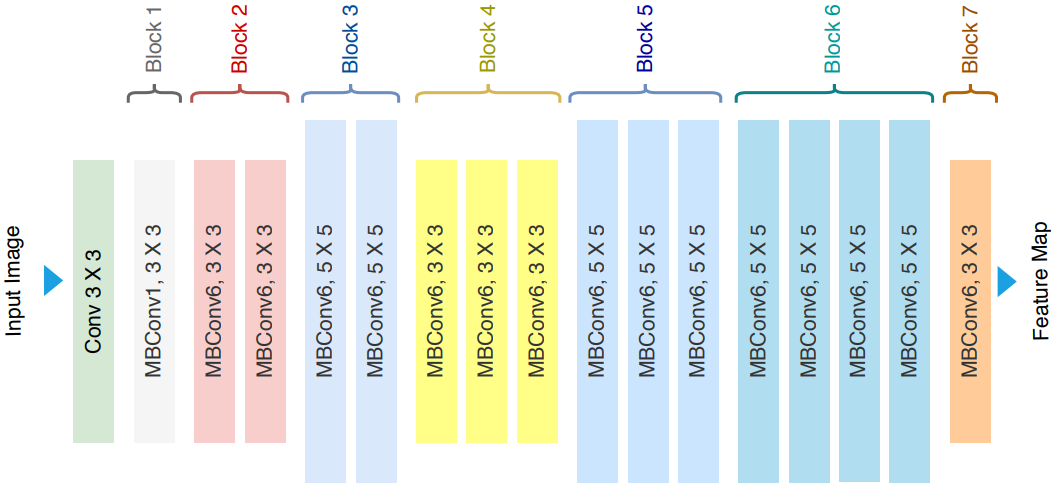
\includegraphics[width=0.6\textwidth]{chapters/chapter1/images/Figure13.png}
    \caption{Architecture of EfficientNet-B0 with MBConv as Basic building blocks \parencite{ahmed2022classification}.}
    \label{fig:figure13}
\end{figure}

\subsubsection{Lightweight and Specialized CNN Models}
Several CNN architectures, such as MobileNet, NASNet, SqueezeNet, and ShuffleNet, have been specifically developed to meet constraints related to speed, model size, and power efficiency, making them suitable for deployment on mobile or edge devices. Although not explored in depth within the main text, a comparative overview of their architectures, key characteristics, and potential applications in smart agriculture is presented in \ref{app:annexA} for further reference.


\section{Transfer Learning and Pretrained Models}
In deep learning, training models from scratch often requires large labeled datasets and significant computational resources. Transfer learning offers a powerful alternative by leveraging models pre-trained on large benchmark datasets such as \textbf{ImageNet}. These pre-trained models capture rich and generalizable features in their initial layers, which can then be adapted to new, often smaller, target datasets with minimal additional training.
This section explores the concept of transfer learning, introduces popular pre-trained CNN architectures relevant to agricultural applications, and outlines fine-tuning strategies suitable for small-scale plant datasets.

\subsection{Concept of Transfer Learning}
Transfer learning is a machine learning technique where a model trained on one task is repurposed for a different but related task. In the context of deep learning, it typically involves taking a neural network pre-trained on a large dataset such as ImageNet, which contains over 14 million labeled images, and adapting it to a specific task that may lack sufficient labeled data.

To formalize this, consider a target learning task \( T_t \) based on a domain \( D_t \); transfer learning allows for assistance from a different domain \( D_s \) for the learning task \( T_s \). The goal of transfer learning is to improve the performance of the predictive function \( f_{T_t}(\cdot) \) for the task \( T_t \) by discovering and transferring latent knowledge from \( D_s \) and \( T_s \), where generally \( D_s = D_t \) and/or \( T_s = T_t \). Furthermore, it is often the case that the size of \( D_s \) is much larger than that of \( D_t \) \parencite{tan2018survey}.

This process is illustrated in Figure~\ref{fig:figure14}, which demonstrates how knowledge from a source task and domain can be transferred to a target task with limited data.

\begin{figure}[H] % 'H' needs \usepackage{float}
    \centering
    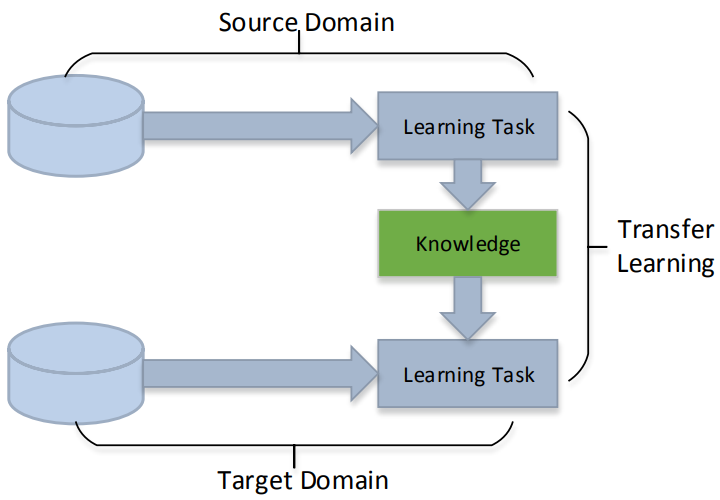
\includegraphics[width=0.6\textwidth]{chapters/chapter1/images/Figure14.png}
    \caption{Learning process of transfer learning \parencite{tan2018survey}.}
    \label{fig:figure14}
\end{figure}
The two primary approaches to transfer learning are \parencite{tan2018survey}:

\begin{itemize}
    \item \textbf{Feature Extraction:} The pre-trained model is used as a fixed feature extractor. All convolutional layers are kept frozen, and only the final fully connected layer(s) are trained on the new dataset.
    \item \textbf{Fine-Tuning:} Some layers of the pretrained model are unfrozen and retrained on the new dataset. This allows the model to slightly adjust its learned features to better suit the new domain.
\end{itemize}

This concept is illustrated in Figure~\ref{fig:figure15}, which demonstrates the integration of a custom CNN with transfer learning networks.

\begin{figure}[H] % 'H' needs \usepackage{float}
    \centering
    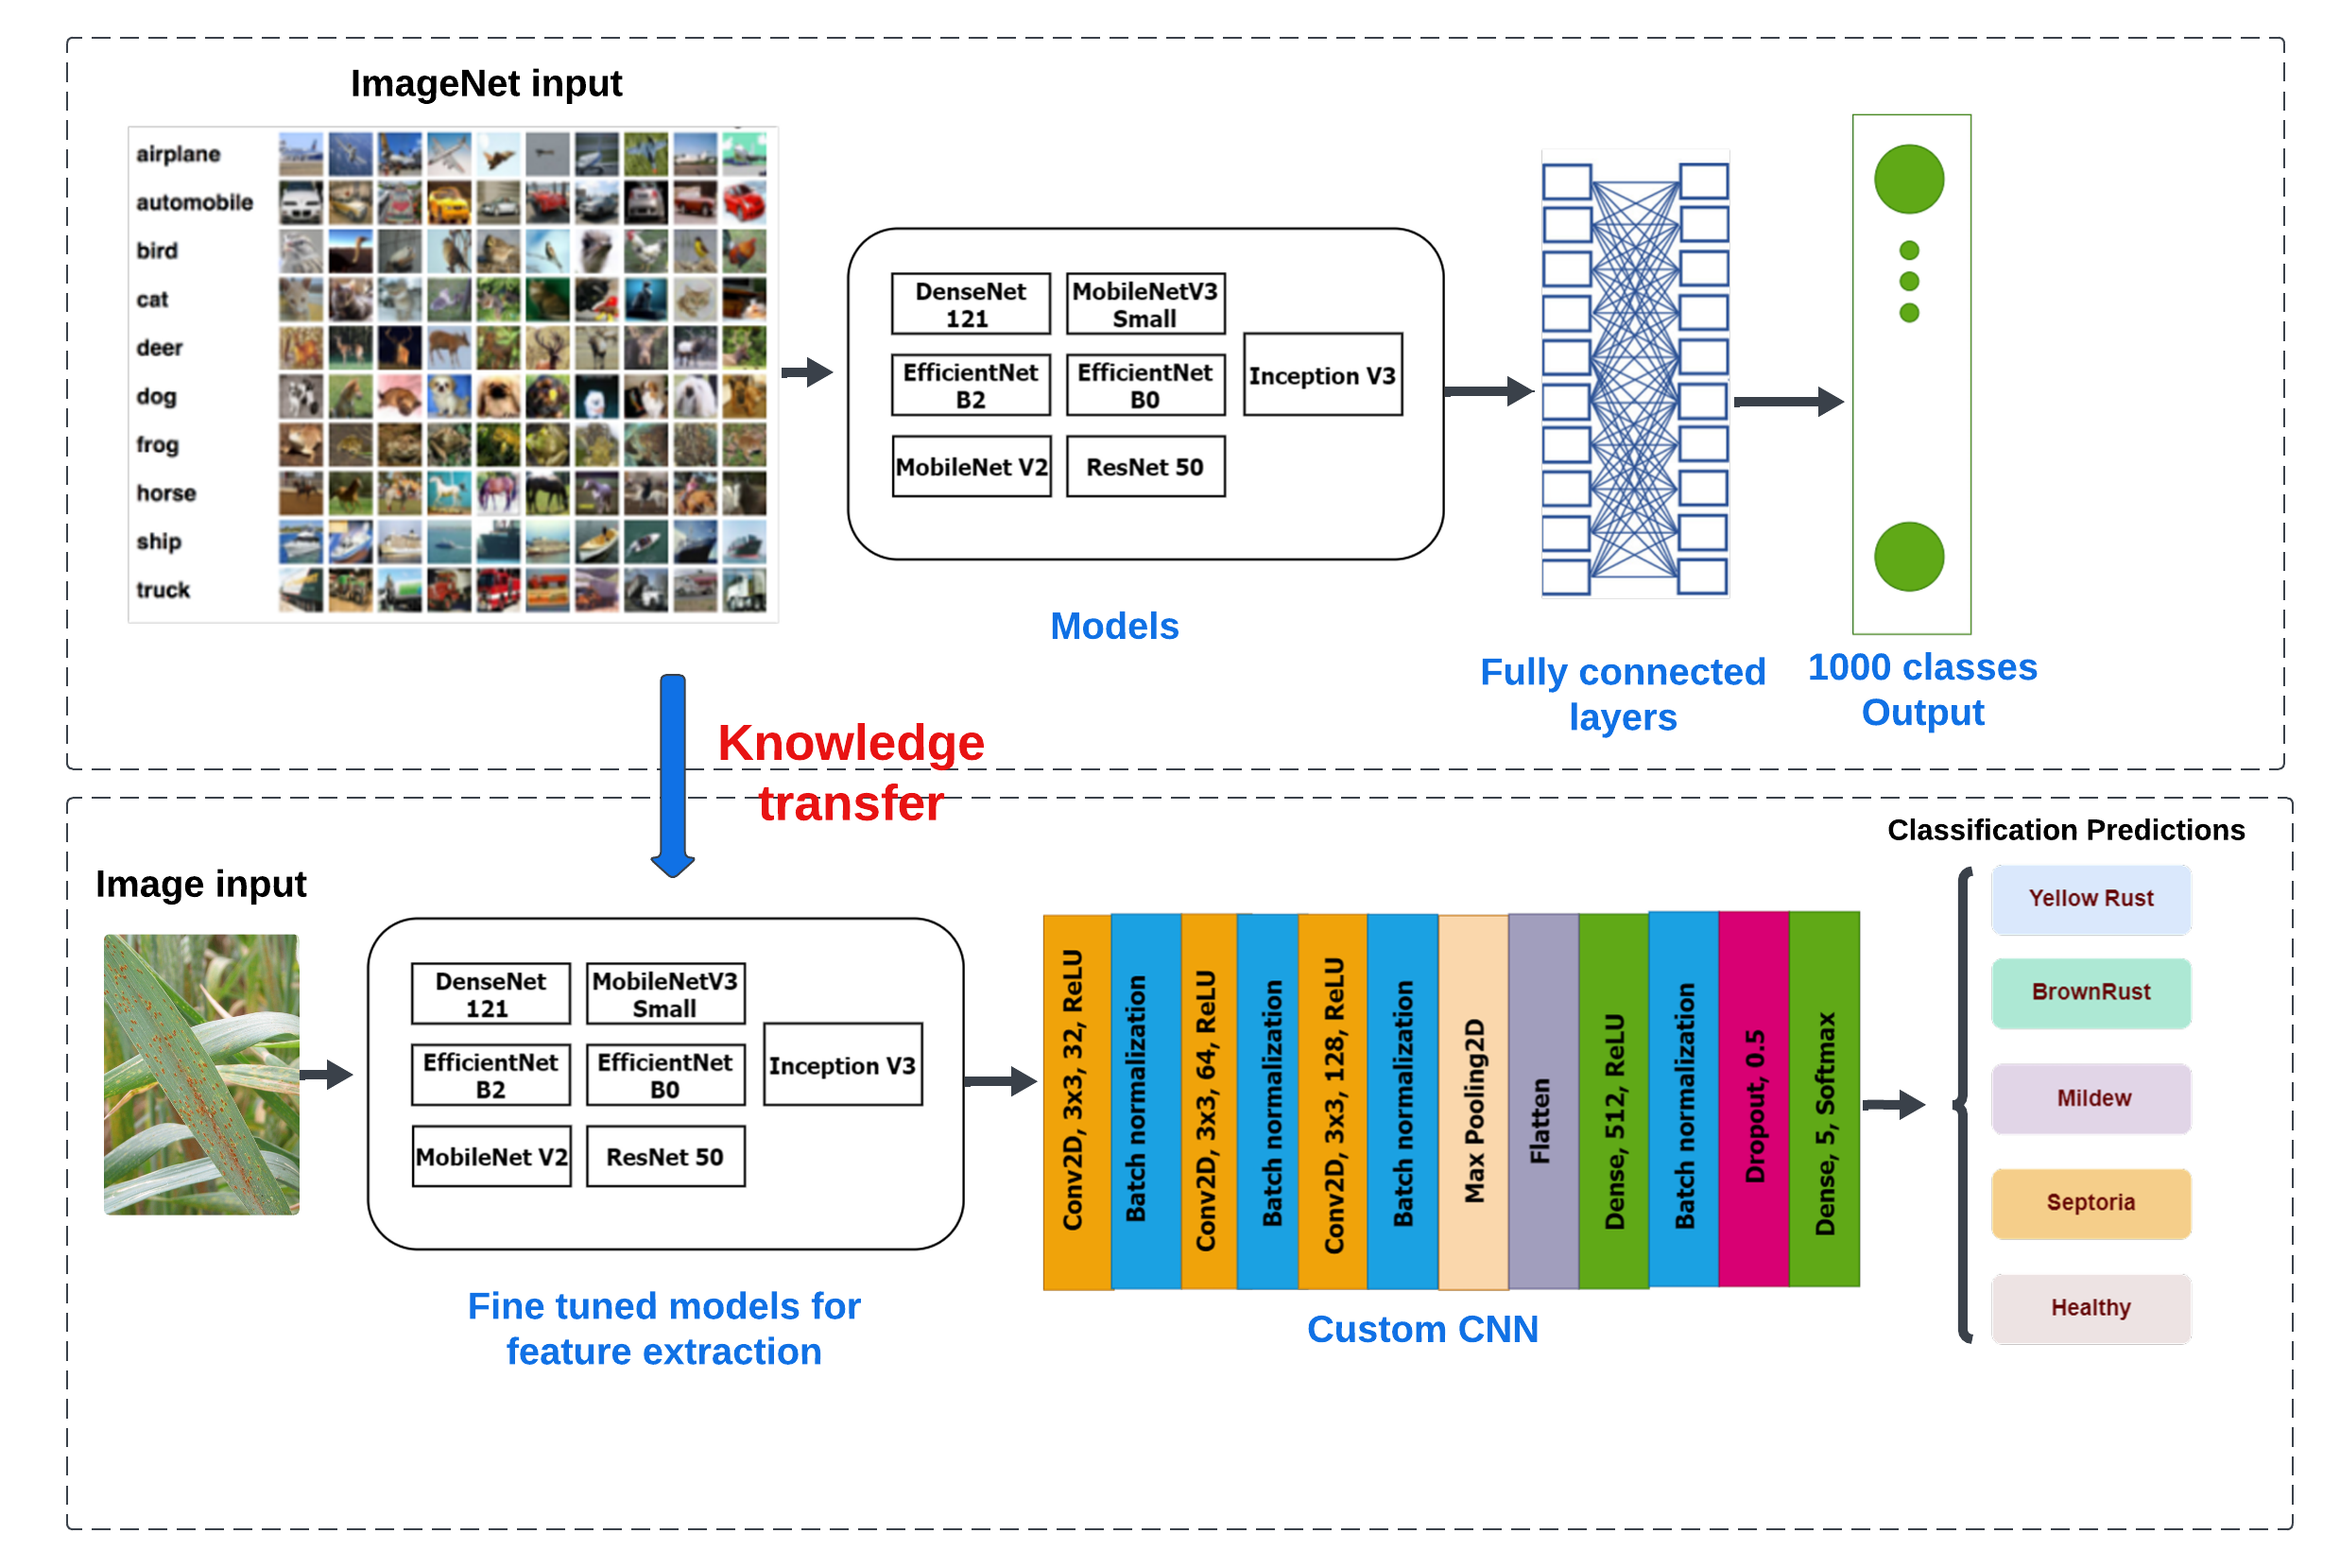
\includegraphics[width=0.8\textwidth]{chapters/chapter1/images/Figure15.png}
    \caption{Integration of the custom CNN with transfer learning networks \parencite{jouini2024wheat}.}
    \label{fig:figure15}
\end{figure}

Transfer learning is especially valuable in agriculture, where acquiring large annotated datasets is difficult. By leveraging pre-trained models, researchers and practitioners can build effective models for plant disease detection with limited data and reduced computational cost


\subsection{Fine-Tuning Strategies for Agricultural Data}


While basic fine-tuning involves unfreezing and retraining a subset of layers in a pretrained model, fine-tuning strategies can be further optimized when dealing with agricultural data, which often presents unique challenges such as class imbalance, limited samples, and high intra-class variability (e.g., similar symptoms across different plant diseases). 

In this context, several fine-tuning strategies can be applied to improve model generalization and performance:
\begin{itemize}
    \item \textbf{Gradual Unfreezing:} Instead of unfreezing all layers at once, layers are incrementally unfrozen, starting from the top (fully connected layers) and moving backward. This helps prevent the model from losing previously learned useful features during early training stages \parencite{hossen2025transfer}.
    \item \textbf{Discriminative Learning Rates:} Assigning different learning rates to different layers, lower for earlier layers and higher for later ones, ensures that the more generic features are preserved while higher-level representations are fine-tuned for the new task \parencite{hossen2025transfer}.
    \item \textbf{Early Stopping and Regularization:} Due to limited data, it's essential to prevent overfitting during fine-tuning. Techniques like early stopping, dropout, and weight decay can help maintain model robustness \parencite{li2021implicit}.
    \item \textbf{Data Augmentation and Balancing:} Supplementing fine-tuning with targeted data augmentation (e.g., rotation, brightness adjustments, zoom) helps the model generalize better. In addition, synthetic oversampling techniques like SMOTE can address class imbalance issues \parencite{aquino2017effect}.
\end{itemize}

These strategies, when integrated thoughtfully, allow researchers to tailor fine-tuning to the specific nature of agricultural datasets, maximizing the benefits of transfer learning even in data-constrained environments.


\section{Object Detection in Smart Agriculture}
In the context of precision agriculture, object detection has emerged as a critical computer vision technique for automating the assessment of crop health. It facilitates the identification and localization of plant diseases, insect pests, nutrient deficiencies, and weeds, supporting more efficient and timely interventions across large-scale farming environments. 
This approach goes beyond simple image classification by offering spatial information about multiple objects of interest within a single image, enabling actionable insights for decision-making.

\subsection{Key Concepts in Object Detection}
Understanding object detection requires familiarity with its key components, including the problem definition, how annotated data is structured, and the metrics used to evaluate model performance. 
\subsubsection{Definition of Object Detection}
At its core, object detection involves predicting both the category and precise location of objects within an image, thus combining classification with localization. Traditional approaches consist of stages such as region proposal, feature extraction, and object classification. Over time, detection methods have evolved to address increasing demands for accuracy and speed, giving rise to both two-stage and one-stage detection frameworks \parencite{zhao2019objectdetection}.

Here are more details about the concepts of object detection \parencite{zhao2019objectdetection}: 
\begin{itemize}
    \item \textbf{Informative Region Selection:} It is used to identify specific areas within an image where objects are likely to appear. This step helps reduce computational load by focusing only on promising regions instead of scanning the entire image at all scales and positions. In agricultural imagery, objects like plants or pests may vary in size, shape, and location. Early methods used multiscale sliding windows to generate candidate regions, but this approach was computationally expensive and often produced redundant proposals. To improve efficiency, modern techniques now use region proposal algorithms or attention mechanisms to better focus on meaningful areas while avoiding irrelevant ones.
    \item \textbf{Feature Extraction:} It is the process of identifying and isolating relevant visual attributes from an image that can effectively represent objects within it. Object recognition involves detecting characteristics that are both robust and semantically significant. Traditional methods such as Scale-Invariant Feature Transform (SIFT), Histograms of Oriented Gradients (HOG), and Haar-like features were designed to mimic human vision by emphasizing edges, textures, and patterns. However, these handcrafted techniques often struggled to maintain performance due to challenges like changes in object appearance, lighting variations, and cluttered backgrounds, leading to their limitations in complex scenarios.
    \item \textbf{Classification and Localization:} Classification and localization refer to the process of both identifying the object in an image and determining its precise location through bounding boxes. With the rise of deep learning, this step underwent a significant transformation. Models such as R-CNN and its subsequent versions—Fast R-CNN, Faster R-CNN, and YOLO—automated the feature extraction process and seamlessly integrated classification with bounding box regression. These advancements led to substantial improvements in both detection accuracy and processing speed, enabling real-time applications in fields like crop monitoring and pest detection.
\end{itemize}

\subsubsection{Annotation of Objects}
Annotation refers to the process of labeling the objects (such as pests, diseases, or damaged crops) in the images by drawing bounding boxes around them and assigning class labels. This is a critical step for supervised learning, where the model learns to identify patterns based on labeled data. Several annotation techniques can be used:
\begin{itemize}
    \item \textbf{Bounding Boxes:} The most common annotation method in object detection. Each object is enclosed in a rectangular box, and the class of the object is assigned to it (e.g., "rust", "aphid").
    \item \textbf{Polygons:} For more precise object delineation, especially when objects have irregular shapes (e.g., plant leaves affected by disease), polygons are used instead of bounding boxes.
    \item \textbf{Semantic Segmentation:} In cases where the task involves classifying each pixel in the image, semantic segmentation labels each pixel to indicate which class it belongs to (e.g., diseased or healthy tissue in a leaf).
\end{itemize}

\subsubsection{Evaluation Metrics in Object Detection}    
In object detection, several metrics are used to assess model performance:
\begin{itemize}
    \item \textbf{Mean Average Precision (mAP):} Measures the average precision across all object classes, balancing precision and recall to evaluate overall model performance.
    \item \textbf{Intersection over Union (IoU):} Calculates the overlap between predicted and ground truth bounding boxes, indicating localization accuracy. Higher IoU means better localization.
    \item \textbf{Precision and Recall:}
    \begin{itemize}
        \item \textbf{Precision:} Measures the proportion of true positive detections out of all predicted objects.
        \item \textbf{Recall:} Measures the proportion of true positive detections out of all actual objects.
    \end{itemize}
    \item \textbf{F1-Score:} The harmonic mean of precision and recall, providing a balance between both.
    \item \textbf{Average Recall (AR):} Evaluates recall at different IoU thresholds, useful for detecting small objects or handling occlusions.
    \item \textbf{Confusion Matrix:} Summarizes true positives, false positives, true negatives, and false negatives, providing insights into model errors.
    \item \textbf{Speed Metrics (FPS, Latency):} Assess real-time performance, essential for time-sensitive applications like precision agriculture.
    \item \textbf{AP at Specific IoU Thresholds:} Measures precision at different IoU levels to understand performance under stricter conditions.
\end{itemize}

\subsection{Key Architectures}
Many architectures are designed to efficiently and accurately detect objects in images, even in complex agricultural environments. Below, we discuss four of the most widely used and effective object detection models: YOLO (You Only Look Once), R-CNN, Faster R-CNN, and SSD (Single Shot Multibox Detector). 

\subsubsection{Yolo}
YOLO is a fast and efficient object detection framework that predicts both object confidences and bounding boxes (BBs) using the entire topmost feature map. The image is divided into a $S \times S$ grid, where each grid cell is responsible for predicting objects centered within it. Each cell predicts multiple bounding boxes and their corresponding confidence scores, which reflect the likelihood of an object being present and how well the predicted box overlaps with the ground truth (IoU) (see figure~\ref{fig:figure16}).

At test time, class-specific confidence scores are computed by multiplying the box confidence with conditional class probabilities. YOLO optimizes a loss function during training to fine-tune predictions and improve detection accuracy \parencite{zhao2019objectdetection}.

\begin{figure}[H] % 'H' needs \usepackage{float}
    \centering
    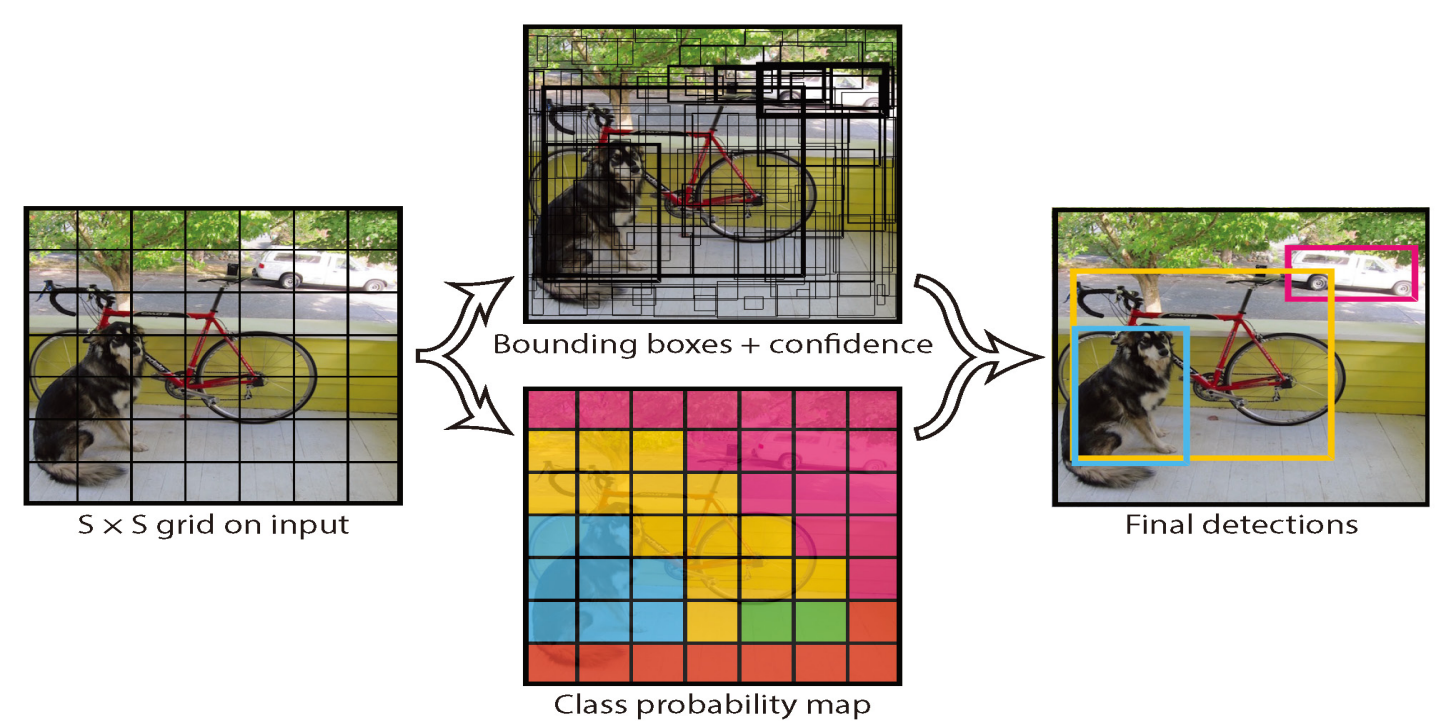
\includegraphics[width=0.7\textwidth]{chapters/chapter1/images/Figure16.png}
    \caption{Main idea of YOLO \parencite{zhao2019objectdetection}.}
    \label{fig:figure16}
\end{figure}

\subsubsection{R-CNN}
R-CNN is a significant advancement in object detection, improving the quality of candidate bounding boxes (BBs) and utilizing deep architecture for high-level feature extraction \parencite{zhao2019objectdetection}. It consists of three main stages, as presented in figure~\ref{fig:figure17}:

\begin{enumerate}
    \item \textbf{Region Proposal Generation:} R-CNN uses selective search to generate about 2000 region proposals per image, improving candidate box accuracy and reducing the search space.
    \item \textbf{CNN-Based Feature Extraction:} Each region proposal is resized and passed through a CNN to extract a 4096-dimensional feature, creating a high-level, robust representation of the object.
    \item \textbf{Classification and Localization:} Region proposals are classified using pre-trained linear SVMs, and bounding box regression is applied. Non-maximum suppression (NMS) is used to eliminate redundant boxes and finalize object detections.
\end{enumerate}

\begin{figure}[H] % 'H' needs \usepackage{float}
    \centering
    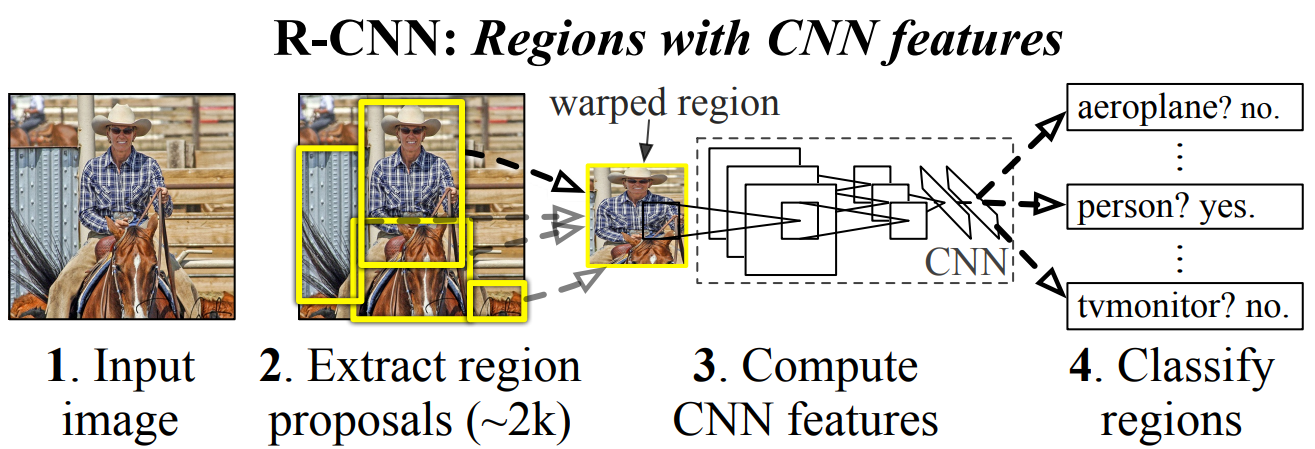
\includegraphics[width=0.7\textwidth]{chapters/chapter1/images/Figure17.png}
    \caption{Flowchart of R-CNN \parencite{zhao2019objectdetection}.}
    \label{fig:figure17}
\end{figure}

Despite its success, R-CNN has drawbacks, including slow inference due to CNN computation for each region, time-consuming multistage training, high memory and storage requirements for storing region features, and redundant region proposals from selective search that slow down the process \parencite{zhao2019objectdetection}.


\subsubsection{Faster R-CNN}


Faster R-CNN improves upon earlier object detection models by introducing a Region Proposal Network (RPN), a deep learning-based method for generating object proposals, which shares convolutional features with the detection network to generate object proposals efficiently, eliminating the need for methods like selective search. The RPN uses a fully convolutional network (FCN) (as presented in Figure~\ref{fig:figure18}) to predict bounding boxes and object scores simultaneously. The system uses anchors of multiple scales and aspect ratios and is trained end-to-end with a multitask loss function. While Faster R-CNN achieves state-of-the-art accuracy and high-speed processing, it is limited by its alternate training algorithm, which is time-consuming and struggles with extreme object scales and shapes \parencite{zhao2019objectdetection}.

\begin{figure}[H] % 'H' needs \usepackage{float}
    \centering
    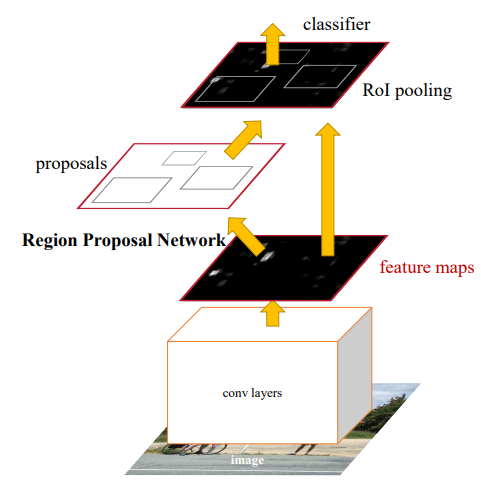
\includegraphics[width=0.6\textwidth]{chapters/chapter1/images/Figure18.png}
    \caption{An illustration of the Faster R-CNN model \parencite{ren2016faster}.}
    \label{fig:figure18}
\end{figure}

\subsubsection{SSD}
SSD was introduced to address the limitations of YOLO, particularly in handling small objects and objects with unusual aspect ratios. Unlike YOLO's fixed grid approach, SSD uses default anchor boxes of various aspect ratios and scales to better handle objects of different sizes.

It integrates predictions from multiple feature maps with different resolutions and uses a VGG16 backbone architecture with additional layers for bounding box predictions. SSD is trained with a combination of localization and confidence losses and refines detections using non-maximum suppression (NMS). It outperforms Faster R-CNN in accuracy on PASCAL VOC and COCO while being three times faster, running at 59 fps with an input size of 300 × 300. However, SSD still struggles with small objects, which can be improved with better feature extractors and network modifications \parencite{zhao2019objectdetection}.

Below is the architecture of SSD (Figure~\ref{fig:figure19}), illustrating its key components, including the VGG-16 backbone, extra feature layers, and classifier convolutions.

\begin{figure}[H] % 'H' needs \usepackage{float}
    \centering
    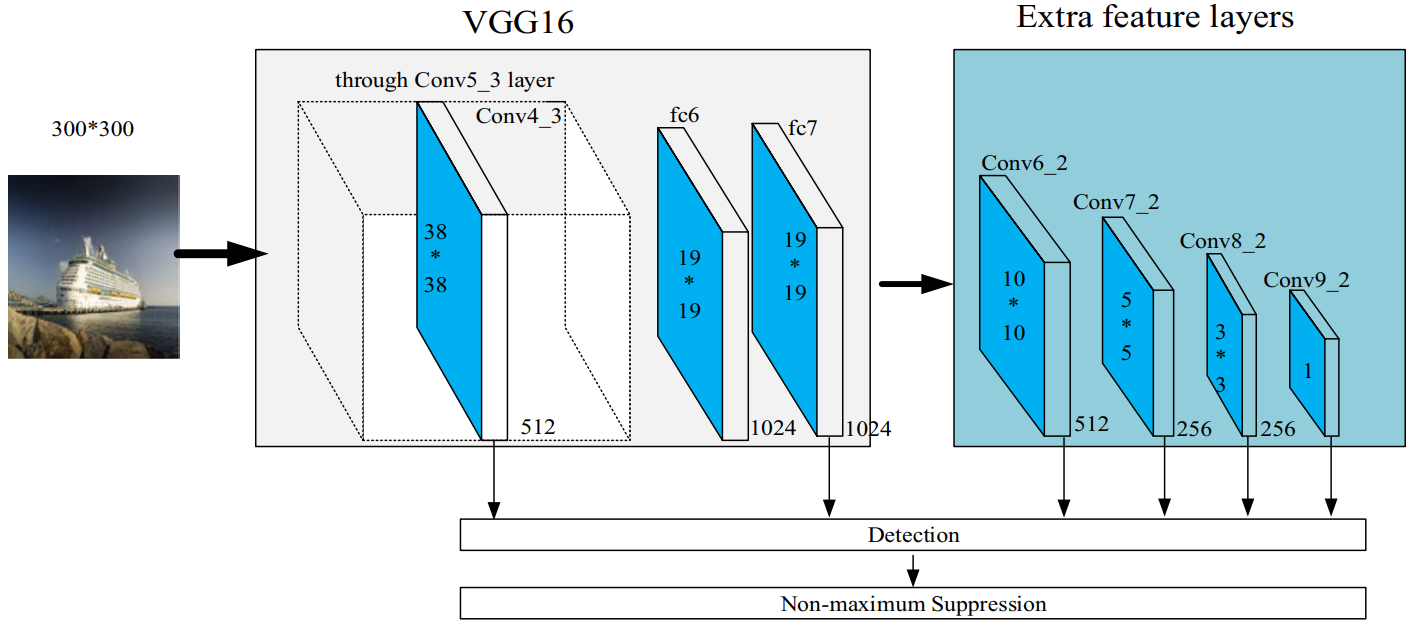
\includegraphics[width=0.6\textwidth]{chapters/chapter1/images/Figure19.png}
    \caption{Architecture of SSD \parencite{li2021water}.}
    \label{fig:figure19}
\end{figure}

\section{Challenges of Deep Learning in Agricultural Contexts}

Despite the promising performance of deep learning and object detection in various fields, their application in agriculture presents a range of specific challenges. One of the primary issues is the limited availability of large, annotated agricultural datasets, which hampers the training of robust and generalizable models. Unlike natural image datasets like ImageNet, agricultural datasets often suffer from class imbalance, incomplete labeling, and domain specificity (e.g., crop types, diseases, and environmental conditions) \parencite{alzubaidi2021review}.

Another challenge is the high intra-class variability and low inter-class variability found in agricultural images. For instance, symptoms of different diseases may look visually similar, or the same disease may appear differently across plant species and growth stages. Additionally, variations in lighting, occlusion by leaves, overlapping plants, and background clutter significantly affect detection performance \parencite{alzubaidi2021review}.

The seasonal and geographic diversity further complicates the generalization of models trained on limited datasets. Moreover, the deployment of deep learning models in real agricultural environments must consider limited computing resources, especially for edge or mobile devices used in fields.

Lastly, ensuring the interpretability and trustworthiness of AI decisions is crucial in agricultural contexts, as these technologies directly impact yield, resource use, and farmers’ livelihoods. Addressing these challenges requires collaborative efforts in data collection, annotation, model adaptation, and efficient deployment strategies \parencite{alzubaidi2021review}.

\section{Conclusion}
In conclusion, this chapter explored the integration of deep learning techniques, especially convolutional neural networks (CNNs), into agricultural contexts, focusing on their role in plant disease classification and object detection. We introduced key CNN architectures such as VGGNet, ResNet, DenseNet, and EfficientNet, each contributing unique design principles and performance improvements. Transfer learning was also discussed as an effective strategy to overcome data scarcity by adapting pretrained models to agricultural datasets with minimal resources.

We then highlighted the concept of object detection and its significance in precision agriculture for tasks like identifying pests, diseases, and weeds. Core ideas such as region proposal, feature extraction, and classification were presented, along with modern deep learning-based solutions. Finally, the chapter addressed real-world challenges, such as image variability, environmental noise, and limited annotated data, all of which must be considered when developing robust AI-based agricultural systems. In the following chapter, we will explore hybrid approaches, such as ensemble learning and its integration with CNN models, to further enhance accuracy, generalization, and robustness in agricultural applications.
